\documentclass{article}
\usepackage{graphics}
\usepackage{pifont}
\usepackage{verbatimbox}
\usepackage{cprotect}
\usepackage{framed}
\usepackage{float}
\usepackage{pdfpages}
\usepackage{tabularx}
\usepackage{array}
\usepackage{amssymb}
\usepackage{cite}
\usepackage{hyperref}
\hypersetup{
    colorlinks=true,
    linkcolor=blue,
    filecolor=magenta,      
    urlcolor=blue,
}
\usepackage{tcolorbox}
\usepackage{xcolor}
\usepackage{fancyvrb}


\usepackage[T1]{fontenc}
\usepackage[utf8]{inputenc}
%%%%This is to indent first paragraph after sectioning.
\usepackage{indentfirst}
% pour les bullets
% utiliser :  \begin {itemize} [label=\textbullet]
\usepackage{enumitem}

%\setlength{\parindent}{0.5cm}

%%ONLY for Xelatex and laulatex...
%\usepackage{fontspec} 
%\usepackage{lilyglyphs} 

\newcommand\bck{$\scalebox{0.6}{$\blacksquare$}~$}

\usepackage[hmargin=3cm]{geometry} 
%\usepackage[dvips,dvipdf]{graphicx}
%\usepackage{landscape}
%\special{landscape} % this allows dvips, dvipdf to "landscape" the document
%\usepackage{multicol}
\geometry{a4paper, portrait}



\usepackage[cyr]{aeguill}
\usepackage[english]{babel}
\usepackage{url}
\let\urlorig\url
\renewcommand{\url}[1]{%
  \begin{otherlanguage}{english}\urlorig{#1}\end{otherlanguage}%
}


%\usepackage{lmodern}             
%\usepackage{imfellEnglish} % I switched to this font 





\usepackage{graphicx,calc}
\newlength\myheight
\newlength\mydepth
\settototalheight\myheight{Xygp}
\settodepth\mydepth{Xygp}
\setlength\fboxsep{0pt}
\newcommand*\inlinegraphics[1]{%
  \settototalheight\myheight{Xygp}%
  \settodepth\mydepth{Xygp}%
  \raisebox{-\mydepth}{\includegraphics[height=\myheight]{#1}}%
}

%\addbibresource{references.bib} % The filename of the bibliography
%\usepackage[autostyle=true]{csquotes} % Required to generate language-dependent quotes in the bibliography

% pour les bullets
% utiliser :  \begin {itemize} [label=\textbullet]
\usepackage{enumitem}
%%%%%%%%Tool for commenting
\newcommand{\trash}[1]{}

\usepackage{verbatimbox}
\usepackage{cprotect}
\usepackage{framed}
\usepackage{float}
\usepackage{pdfpages}
\usepackage{harmony}
\usepackage{arcs}
\usepackage{qtree}
\usepackage{mathtools}
\usepackage{xargs}
\usepackage{csquotes}%for doublequotes in biblio

%\usepackage{verse}
\usepackage{attrib}


\usepackage{graphicx}
\newcommand{\unaryminus}{\scalebox{0.5}[0.72]{\( - \!\)}}

\begin{document}
%\setlength{\parindent}{0.8cm}
\setlength{\parskip}{0.3cm}


\title{omlily}
\author{Karim Haddad}
\date{\today}
\maketitle

\section{About}

omlily\cite{haddad2016omlily} is an OpenMusic\cite{bresson2011openmusic} Library interfacing with Lilypond\cite{nienhuys2003lilypond} the music engraving program. 

\section{Compatibility}

This Library is compatible with OpenMusic 6.x and runs on Linux, MacOsX and Windows platforms.

\section{Installation}

Install the folder 'omlily 3.x' in your OpenMusic Library's desired path. 


\subsection{Linux} 

Once loaded, the library will automatically query the Lilypond binary in your path. For Linux users, it will also query for the xpdf reader. You can change these options in OpenMusic preferences in the External tab. For MacOsX and Windows users, the default system pdf reader will be used for displaying the score.


\subsection{Macosx}


In order to have the library automatically compile your *.ly file, you will need, beside the standard installation of Lilypond.app, to configure the command-line link to the application as described here in the "Running on the command-line": \url{http://www.lilypond.org/website/macos-x.html}



\subsection{Windows}


In order to have the library automatically compile your *.ly file, you will need, beside the standard installation of Lilypond.exe, to configure the command-line link to the application as described here in the "Running on the command-line": \url{http://lilypond.org/website/windows.html}



\section{Usage}



\subsection{OM->LILY}

om->lily will export and compile VOICE, POLY, CHORD-SEQ and MULTI-SEQ objects into lilypond *.ly files.

\subsubsection{Modes}
om->lily has two basic modes for generating the score according to the nature of the polyphony:

\begin{description}
   \item [\textbullet~ Generic :] for most of the music that is set without polymetrics and polytempi.
   \item [\textbullet~ Polymetric :] for special cases where music is polymetric and/or polytempic. 
\end{description}


%\subsubsection{Structure of the *.ly file}
%The basic structure of a *.ly file exported with om->lily method is structured in multiple blocks:


\subsection{LILY->OM}

In order to import *.ly files into OpenMusic objects (POLY), you will have to:\\
\begin{enumerate}
\item Uncomment the following 3 lines found in your *.ly generated file:\\

\begin{tcolorbox}
  
\begin{verbatim}
\score { 
 { 

...


% #(with-output-to-file "temp.lisp" --> uncomment
% (lambda () #{ \displayMusic {     --> uncomment

...

% } #}))   --> uncomment

} 
\end{verbatim}    

\end{tcolorbox}  
\vskip 5pt

\item After removing the comment sign '\%', you should recompile your file with Lilypond. This will produce a "temp.lisp" file.\\

\item Connect lily->om to the first input of a POLY object (<self>) or CRTL+SHIFT+CLICK the output of lily->om in order to create a POLY instance.\\

\end{enumerate}

Important:

The Lilypond/Openmusic communication will work ONLY with om->lily generated files. 

"barchecks" are mandatory. If they are absent this will output erroneous rhythms.

If not, please be really carefull when:\\

\begin{enumerate}
%\item In case of a single voice, or a single PianoStaff to group them between \guillemotleft~ and \guillemotright~ in the Score section.\\

\item For general cases of music, put bar checks after each measures.\\

\item In case of PianoStaff cross-staff notation, this will not render as a cross-staff in OM. Hence all notes will stay on the same staff.

\item PianoStaff is not yet integrated nor the CHORD-SEQ export.

\item Polymetric and tempo changes are not yet supported.

\end{enumerate}

\section{Preferences}

\begin{figure}[H]
    \centering
    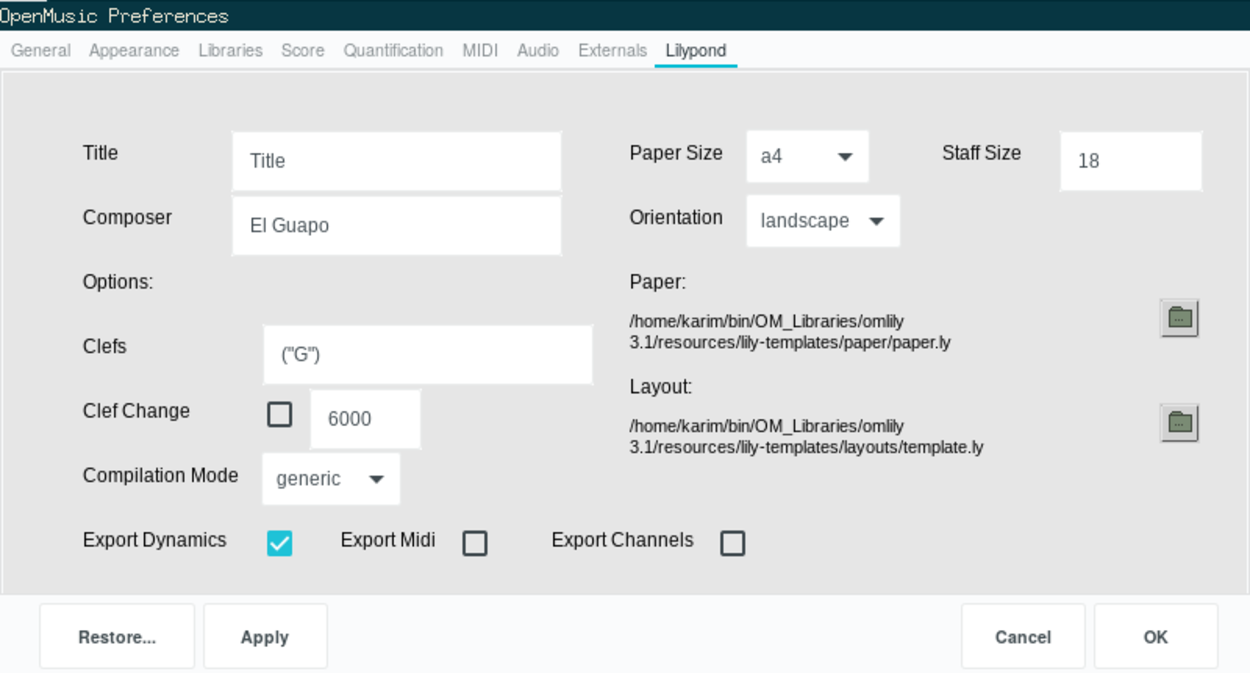
\includegraphics[scale=0.7]{fig/panel}
    %\caption{ 
    %  \label{fig:form001}
    %}
  \end{figure}
  

The preference panel under the Lilypond tab:\\
%\begin{itemize}[label=\textbullet]
\begin{description}
\item [\textbullet~ Title :]	 sets the title of the score.

\item [\textbullet~ Composer :] sets the composer's name of the score.

\item [\textbullet~ Options :] \phantom{}
  \begin{description}
  \item [\bck Clefs :]  sets the clefs. 
  \item [\bck Clef Change :] sets the switching of clefs between G and F (in midicents). 
  \item [\bck Compilation mode :] sets the compilation mode generic/polymetric according to the given music.
  \item [\bck Export Dynamics :] if checked, dynamics will be exported.
  \item [\bck Export Midi :] if checked, will export a midi file.
  \item [\bck Export Channels :] if checked, all midi channels will be displayed as fingerings.
  \end{description}

\item [\textbullet~ Paper Size :] sets the paper size a4/a3.

\item [\textbullet~ Staff Size :] sets the global staff size.

\item [\textbullet~ Orientation :] sets paper orientation between portait/landscape.

\item [\textbullet~ Paper :] Choose a template for more specific paper preferences (margins, page numbering, ...)

\item [\textbullet~ Layout :] Choose a template for most Lilypond specific preferences and contexts.

\end{description}

The preferences will be saved in a future session of the workspace ONLY if the library is set in \textit{autoload} mode (cf. OM documentation).
\appendix
\section{Appendix}

om->lily output default file example:

\begin{verbatim}

\version "2.19.83"

#(set-default-paper-size "a4landscape")
#(set-global-staff-size 18)
\paper {
    system-system-spacing = #'((basic-distance . 15) (padding . 20))
     system-separator-markup = \slashSeparator
    #(define after-title-space (* 0.5 cm))
    #(define head-separation (* 0.5 cm))
    print-page-number = ##t
    print-first-page-number = ##t
    first-page-number =#1
   top-margin = 2\cm
   bottom-margin = 3\cm
         two-sided = ##t
   inner-margin = 20\mm
   outer-margin = 20\mm
%%%%%these come together:%%%%
    %left-margin = 20\mm
    %line-width = 380\mm
%%%%%%%%%%%%%%%%%%%%%%%%%%%%% 
  tagline = \markup {

  }
}





\header {
breakbefore =##t
title = \markup {"Title"}
composer = \markup {"El Guapo"}
}

 
"one"=
{
%%%%%%%%%%%%%%%%%%%%%%%%%%%%%%%%%%%%%%%%%%%%%%%%%%%%%%%%%%
%%%%%%%%%%%%%%%%%%%%%%% VOICE : 1 %%%%%%%%%%%%%%%%%%%%%%%%
%%%%%%%%%%%%%%%%%%%%%%%%%%%%%%%%%%%%%%%%%%%%%%%%%%%%%%%%%%


#(set-accidental-style 'dodecaphonic)

\clef "G"
%%%%%%%%%%%%%%%%%%%%%%% MESURE : 1 %%%%%%%%%%%%%%%%%%%%%%%
\tempo 4 = 60
\time 4/4
c'4 \f
c'4
c'4
c'4
|
} 
 

\score { 
 { 


<<
% #(with-output-to-file "temp.lisp"
% (lambda () #{ \displayMusic { 

\new StaffGroup
 << 


\new Staff  {
\one
}


 >> 


 % } #}))


 >>

} 
 

%%%%%%%%%%%%%%%%%%%%%%%%%%%%%%%%%%%%%%%%%%%%%%%%%%%%%%%%%%%%%%%%%%%%%%%%%%%%%%
%%%%%%%%%%%%%%%%%%%%%%%%%%%%%%%%omlily template%%%%%%%%%%%%%%%%%%%%%%%%%%%%%%%
%%%%%%%%%%%%%%%%%%%%%%%%%%%%%%%%%%%%%%%%%%%%%%%%%%%%%%%%%%%%%%%%%%%%%%%%%%%%%%





\layout {
	ragged-last = ##f
indent = 0.0
\context {\Score 
         \override TupletBracket #'staff-padding = #1.5
         \override TupletBracket #'direction = #1
         \override TupletBracket #'bracket-visibility = ##t
          \override Stem #'stemlet-length = #0.75
	  \remove "Mark_engraver" %%%for the fermata on barline 
	   \override MetronomeMark #'padding = #2.5
	  %\remove "Timing_translator"
	  %\remove "Default_bar_line_engraver"

         }
\context {\Staff
         \numericTimeSignature
          \override NoteHead #'style = #'baroque
	   \override DynamicLineSpanner #'staff-padding = #3  %%add this by default Should I ??
\override Flag #'stencil = #modern-straight-flag
	   \consists "Mark_engraver" %%%for the fermata on barline
       %   \consists "Timing_translator"
	%  \consists "Default_bar_line_engraver"

}
}
}


\end{verbatim}

\bibliography{omlily_doc}{} 
\bibliographystyle{plain}
\end{document}
